This section briefly explains the medicine RS research area, lists similar
systems, and explains what technologies their researchers used to build
them. When available, we also try to look into their solutions for the
objectives listed in section \ref{AimObjectives}. We will split the
research into two categories, described in the following subsections.

\subsection{Ontology and Rule-Based Systems}

These systems typically rely on a set of rules, referred to as a knowledge
base, that mimic the logic of a medical expert \cite{Stark2019}.

GalenOWL \cite{Doulaverakis2012} recommends drugs to patients based on the
user's diseases, allergies and drug interactions. The system stores the
rules in a Resource Description Framework graph and uses SPARQL to query
the knowledge space. The results were reviewed and evaluated by a medical
expert, and it was stated in future work that there should be an expansion
of semantic rules. 

Doulaverakis et al. created the Panacea \cite{Doulaverakis2014} system based on
GalenOwl's approach. They use SKOS vocabulary for the rules. Results show
better query performance over GalenOwl and accommodate a far greater knowledge
base.


Lakkaraju et al.\cite{pmlr-v54-lakkaraju17a} model their RS using a decision list
as a Markov Decision Process (MDP) and Upper Confidence Bound Trees to
prune the search space efficiently. Their system maps between demographics
and treatments and try to maximise outcomes, minimise treatment costs and
expresses this into an interpretable tree-based model. They evaluated
their system by using criminal justice and health care domains. 


Not all medical RS focus on recommending medicine to all types of
patients; some decide to focus on a specific group of people. For example,
IRS-T2D \cite{Mahmoud2016} is a system built to personalise medicine for
patients with type 2 diabetes. The solution uses Semantic Web Rule Language
from HbA1c  tests, anti-diabetics, and dose selection restrictions. To evaluate
their system, they used a dataset made up of 30 patients and achieved a very
high precision rate. 

Hamed et al. \cite{Hamed2012} make a different approach. They analyse a set of
500,00 tweets to recommend medication. They start by checking the condition of
a person, send them a questionnaire to get more info and apply a C4.5 decision
tree algorithm to predict the condition of the user. Based on the result, the
algorithm can derive the correct medical product. 

While rule-based approaches offer reasonable solutions, they also have
advantages and disadvantages. Since everything is based on rules, they are
more prone to cold start issues \cite{PradeepKumarSingh2021}. However, They are
not easy to scale, and it is challenging to add rules to an ample domain space
without introducing conflict \cite{Bhoi2021}.

\subsection{
Machine learning-based Approaches
}

There are two main ways of approaches to building Machine-Learning based
RS. The first method is using Collaborative Filtering (CF). Using this
approach, an RS recommends items to a user based on the choices of similar
users. The algorithm measures user similarity from features like
demographics, diagnosis or prescriptions. Another approach is using
content-based filtering (CF), which uses item similarity instead. For
example, if a user was given medicine A with similar features to medicine
B, that is recommended. 

CF is used by CADRE \cite{Zhang2015}, trained on the Walgreens dataset, which unfortunately has been removed. CADRE is a cloud-based RS that performs top-N recommendations in three steps. The data pre-processing
part is for clustering and cleaning the data, and after CF, tensor
decomposition addresses the sparsity problem of CF. Unfortunately, this
system achieved low results; however, not many features were used to train
the model, and the dataset contains only around 6000 users. They state
that future work could use user demographics to increase F1, accuracy and
recall scores.

The Mimic dataset is a publicly available EHR dataset that will be
described in detail later in section X. Several RS use such datasets like
LEAP, PREMIER and Wang et al.'s system. 


Zhang et al. \cite{LEAP} created LEAP , an end-to-end learning algorithm that uses a
recurrent decoder and content-based attention for treatment recommendation from
disease-drug mapping. Leap used reinforcement learning to fine-tune the model
and achieved a 10\% increase performance overall baselines. Bhoi et al. 
\cite{Bhoi2021} categorised this approach as an instance-based system that
only recommends medicine based on current visits and does not consider past
visits. 

\begin{figure}
    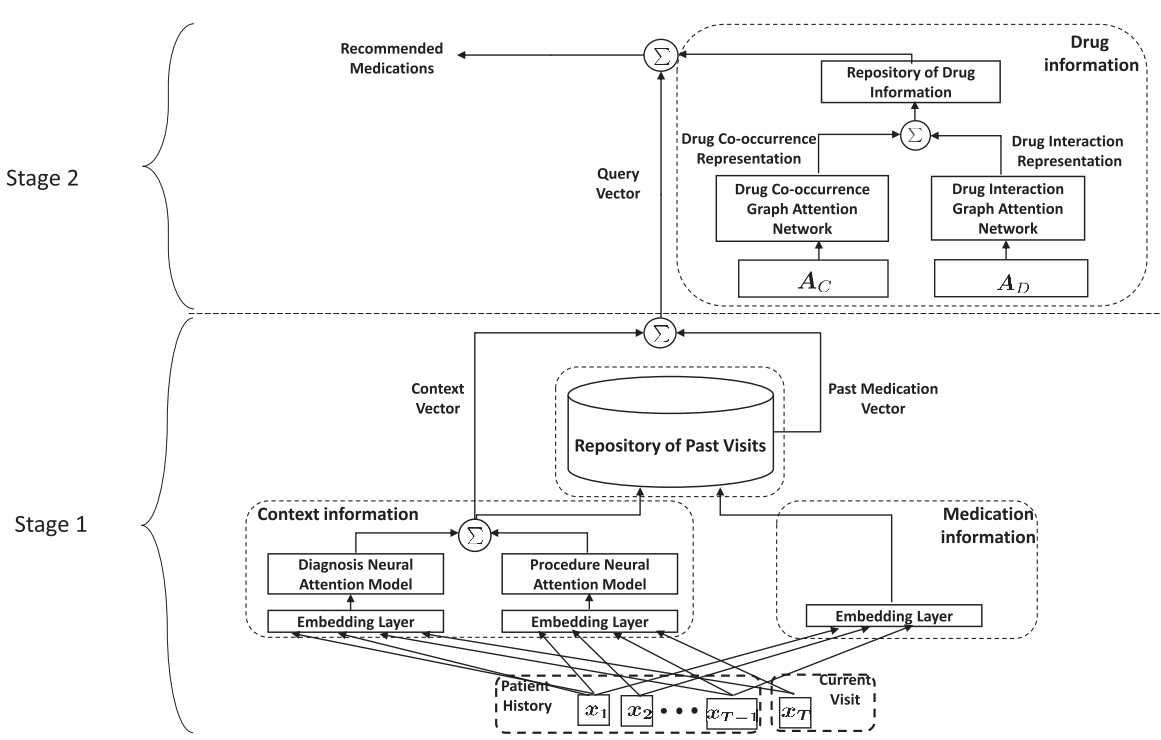
\includegraphics[width=8.5cm, height = 7.5cm]{PREMIER.png}
    \caption{PREMIER's two Stage Recommender System.}
    \label{one}
\end{figure}

Recurrent Neural Networks were popular architectural choices for mimic-based RS
mainly because of their memory ability which is vital for training on user
visits \cite{Wang}. PREMIER \cite{Bhoi2021} is a two-stage attention-based
RS. Figure \ref{one} shows the architecture with information about each stage. In
the first stage, the system uses past diagnoses and procedures and embeds
this information into the RNN. In the second stage, they combine the
second dataset of drug interactions to ensure that each recommendation is
safe for the user. The system also justifies the recommendations by
splitting them into two parts; one for the diagnosis and one for the
procedures, and uses a weight feature to calculate the importance. As a
result, PREMIER outperforms state-of-the-art medication recommendation
systems while achieving the best tradeoff between accuracy and drug-drug
interaction.  

Finally, Wang et al. \cite{Wang} proposed a solution that uses Supervised Reinforcement
Learning with RNNs on the Mimic Dataset. They contain an off-policy
actor-critic architecture to discover unique optimal personalised
treatments and evaluated that their system can decrease the estimated
mortality in hospitals by up to 4.4\%.

